\section{CUI AMT332S-V ABN-Encoder}\label{Appendix:ABC_Ecoder}

\subsection{Pinout and Interface}

\begin{figure}[H]
	\centering
	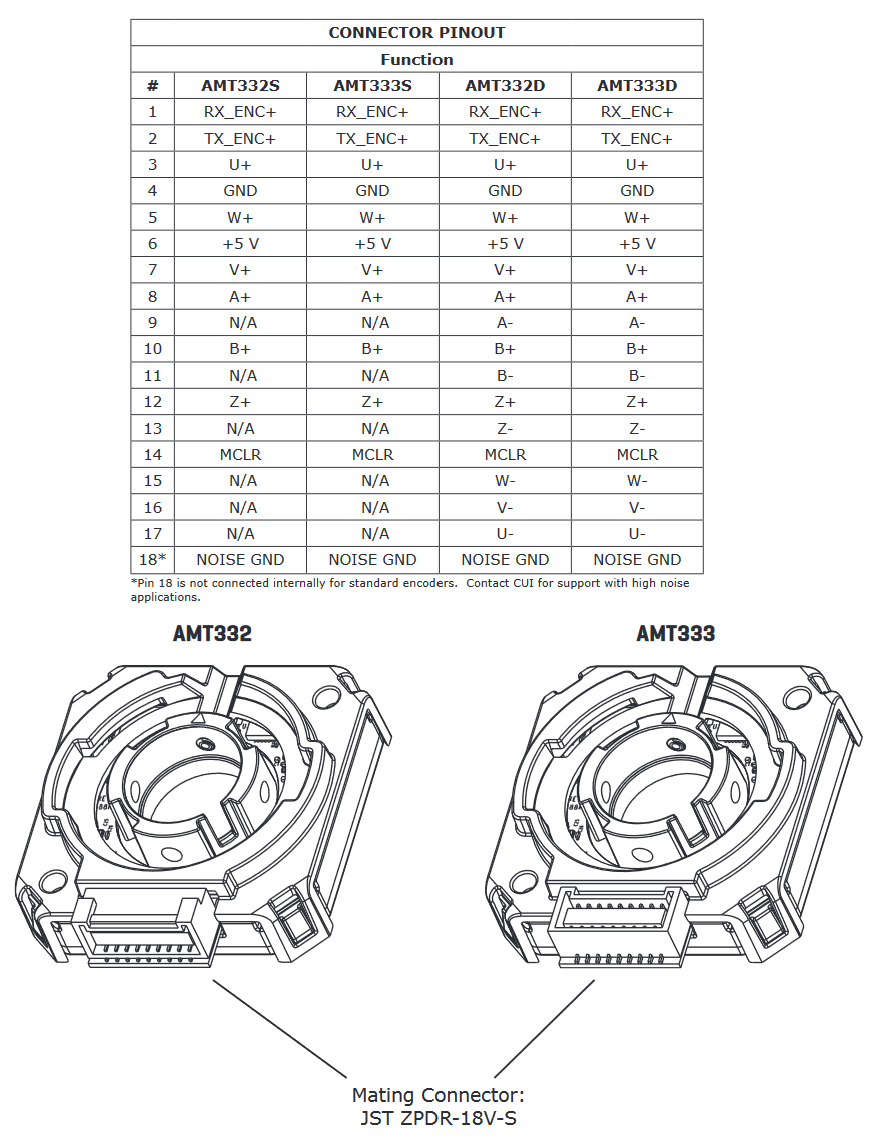
\includegraphics[width=\textwidth]{graphics/Encoder_Interface}
	\caption{Encoder-Interface Pinout-Table.\cite[S.5]{cui_devices_cui_2019}}
	\label{fig:Encoder_Interface}
\end{figure}

\newpage

\subsection{Inbetriebnahme}

\subsubsection{Register}\label{Appendix:ABN_Register}

\begin{table}[H]
\begin{tabularx}{\linewidth}{|l|l|l|X|}
\hline
\multicolumn{4}{|c|}{\textbf{TMC4671 Register}}               \\ \hline
\textbf{Nr. }& \textbf{Register-Name   }   & \textbf{Wert }      & \textbf{Was} \\ \hline
\multicolumn{4}{|l|}{\textbf{Motor type \&  PWM configuration}}        \\ \hline
0x17         & PWM\_POLARITIES             & 0x00000000 & MOSFETs polarity ''off''    \\ \hline
0x1B         & MOTOR\_TYPE\_N\_POLE\_PAIRS & 0x00030003 &     \\ \hline
0x18         & PWM\_MAXCNT                 & 0x00000F9F & PWM frequency 25kHz = 100MHz/(3999+1)   \\ \hline
0x19         & PWM\_BBM\_H\_BBM\_L         & 0x00001919 & Break-before-Make-Time[10ns] MOSFET gate control \\ \hline
0x1A         & PWM\_SV\_CHOP               & 0x00000007 & PWM chopper mode: centtered PWM for FOC \\ \hline
\multicolumn{4}{|l|}{\textbf{ADC configuration}}                       \\ \hline
0x0A         & ADC\_I\_SELECT              & 0x24000100 & ADC\_I0\_(RAW), ADC\_I1\_(RAW)    \\ \hline
0x04         & dsADC\_MCFG\_B\_MCFG\_A     & 0x00100010 & (TMCL-IDE)    \\ \hline
0x05         & dsADC\_MCLK\_A              & 0x20000000 & (TMCL-IDE)    \\ \hline
0x06         & dsADC\_MCLK\_B              & 0x00000000 & (TMCL-IDE)    \\ \hline
0x07         & dsADC\_MDEC\_B\_MDEC\_A     & 0x014E014E & (TMCL-IDE)    \\ \hline
0x09         & ADC\_I0\_SCALE\_OFFSET      & 0xFF0080CF & (TMCL-IDE)    \\ \hline
0x08         & ADC\_I1\_SCALE\_OFFSET      & 0xFF008E04 & (TMCL-IDE)    \\ \hline
\multicolumn{4}{|l|}{\textbf{ABN-Encoder settings}}           \\ \hline
0x25         & ABN\_DECODER\_MODE            & 0x0000100A & Pins = A,B,N, polarities = 0,1,0, direction = 1    \\ \hline
0x26         & ABN\_DECODER\_PPR             & 0x00002000 & Pulses per mechanical revolution = 8192 \\ \hline
0x27         & ABN\_DECODER\_COUNT           & 0x00000000 & Decoder count start = 0 \\ \hline
0x29         & ABN\_DECODER\_PHI\_E\_PHI\_M\_OFFSET  & 0x00000000 & Angle = 0    \\ \hline
\multicolumn{4}{|l|}{\textbf{Limits}}                         \\ \hline
0x5C         & PID\_TORQUE\_FLUX\_TARGET\_DDT\_LIMITS & 0x00007FFF & $\frac{di}{dt}$ Maximale Änderung Drehmoment/Fluss   \\ \hline
0x5D         & PIDOUT\_UQ\_UD\_LIMITS         & 0x00005A81 &    Maximaler Regelfehler UQ/UD 23'169\\ \hline
0x5E         & PID\_TORQUE\_FLUX\_LIMITS      & 0x000009C4 &    Maximales Drehmoment/Fluss = 2500mA\\ \hline
0x5F         & PID\_ACCELERATION\_LIMIT      & 0x000000C8 & Maximale Beschleunigung = 200     \\ \hline
0x60         & PID\_VELOCITY\_LIMIT          & 0x000005DC & Maximale Geschwindigkeit = 1500    \\ \hline
0x61         & TMC4671\_PID\_POSITION\_LIMIT\_LOW & 0x80000001 &    Unterer Positionslimit = -2'147'483'649 \\ \hline
0x62         & PID\_POSITION\_LIMIT\_HIGH     & 0x7FFFFFFF & Oberes Positionslimit = 2'147'483'648  \\ \hline
\multicolumn{4}{|l|}{\textbf{PI-Settings}}       \\ \hline
0x56         & PID\_TORQUE\_P\_TORQUE\_I    & 0x00642EE0 &  Drehmoment: P = 100 / I = 12'000   \\ \hline
0x54         & PID\_FLUX\_P\_FLUX\_I  & 0x00642EE0 &  Fluss : P = 100 / I = 12'000   \\ \hline
0x58         & PID\_VELOCITY\_P\_VELOCITY\_I  & 0x07D001F4 & Geschwindigkeit: P = 2000 / I = 500    \\ \hline
0x5A         & PID\_POSITION\_P\_POSITION\_I  & 0x00C80000 & Position : P = 200 / I = 0    \\ \hline
\end{tabular}
\end{table}

\subsubsection{Inbetriebnahme Setup}\label{Appendix:ABN_Setup}

\begin{figure}[H]
	\centering
	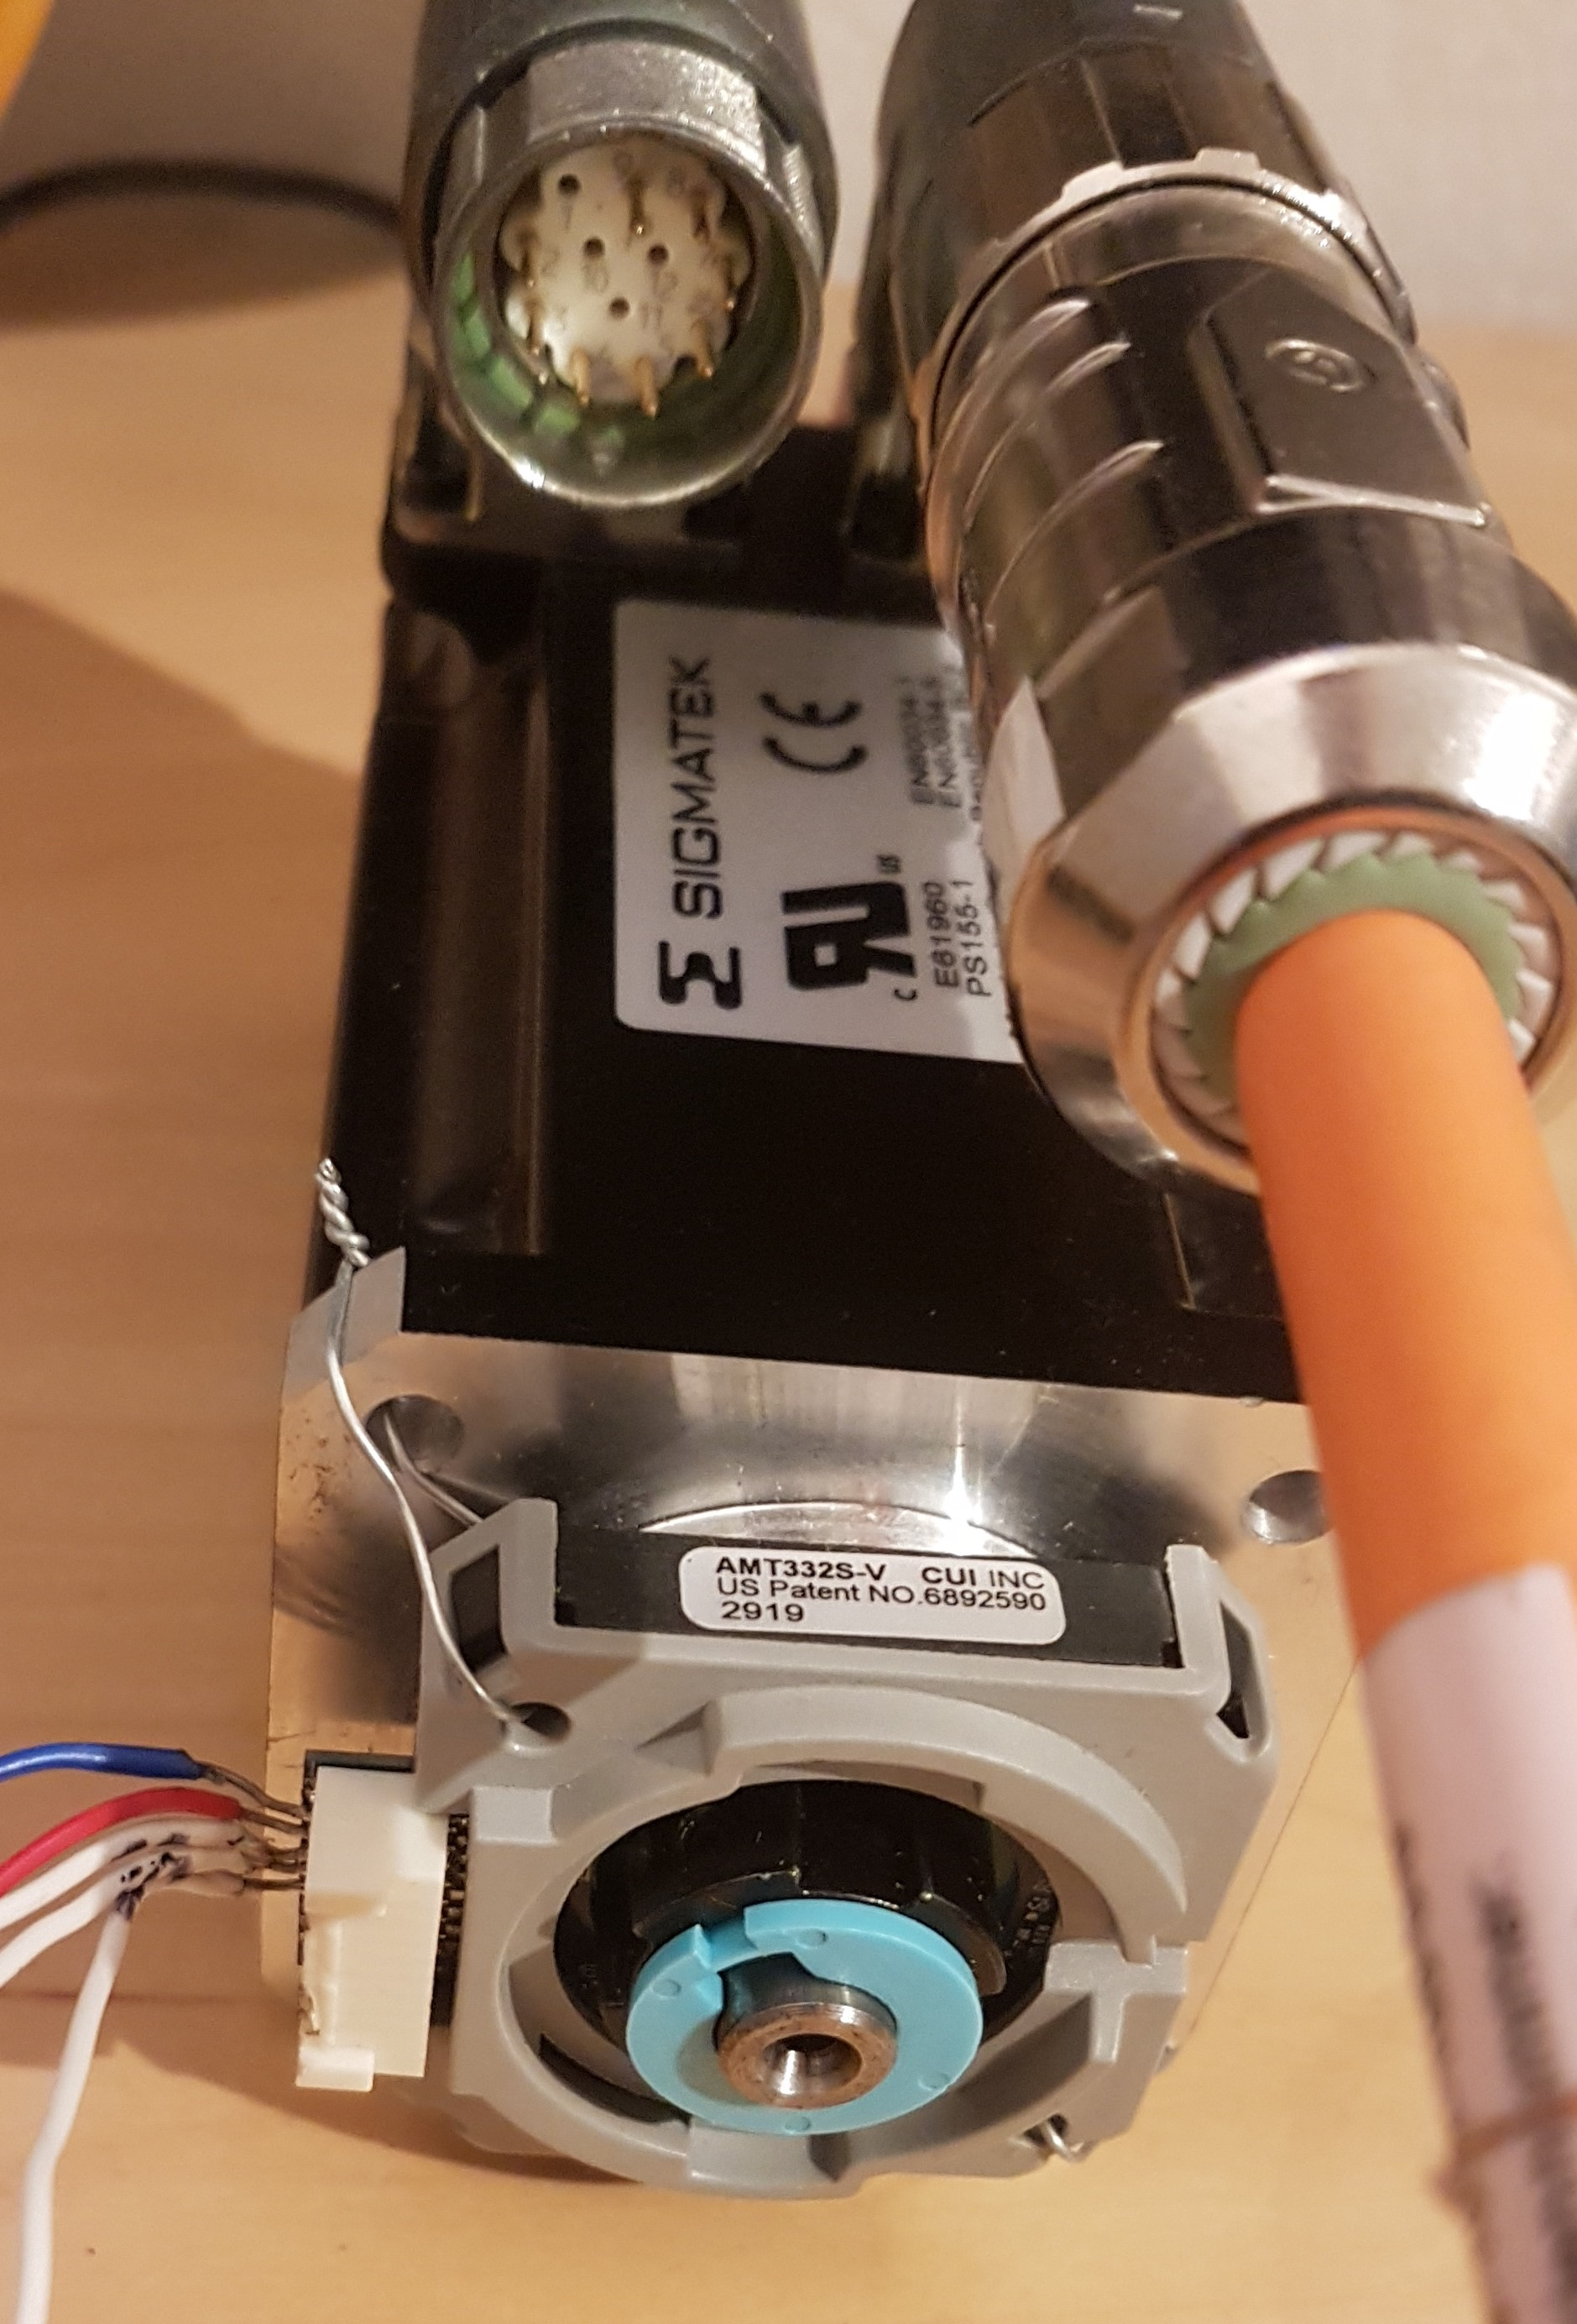
\includegraphics[angle = 270, width=\textwidth]{graphics/4_Encoder_Motor}
	\caption{Encoder-Interface Pinout-Table.}
	\label{fig:4_Encoder_Motor}
\end{figure}

\begin{figure}[H]
	\centering
	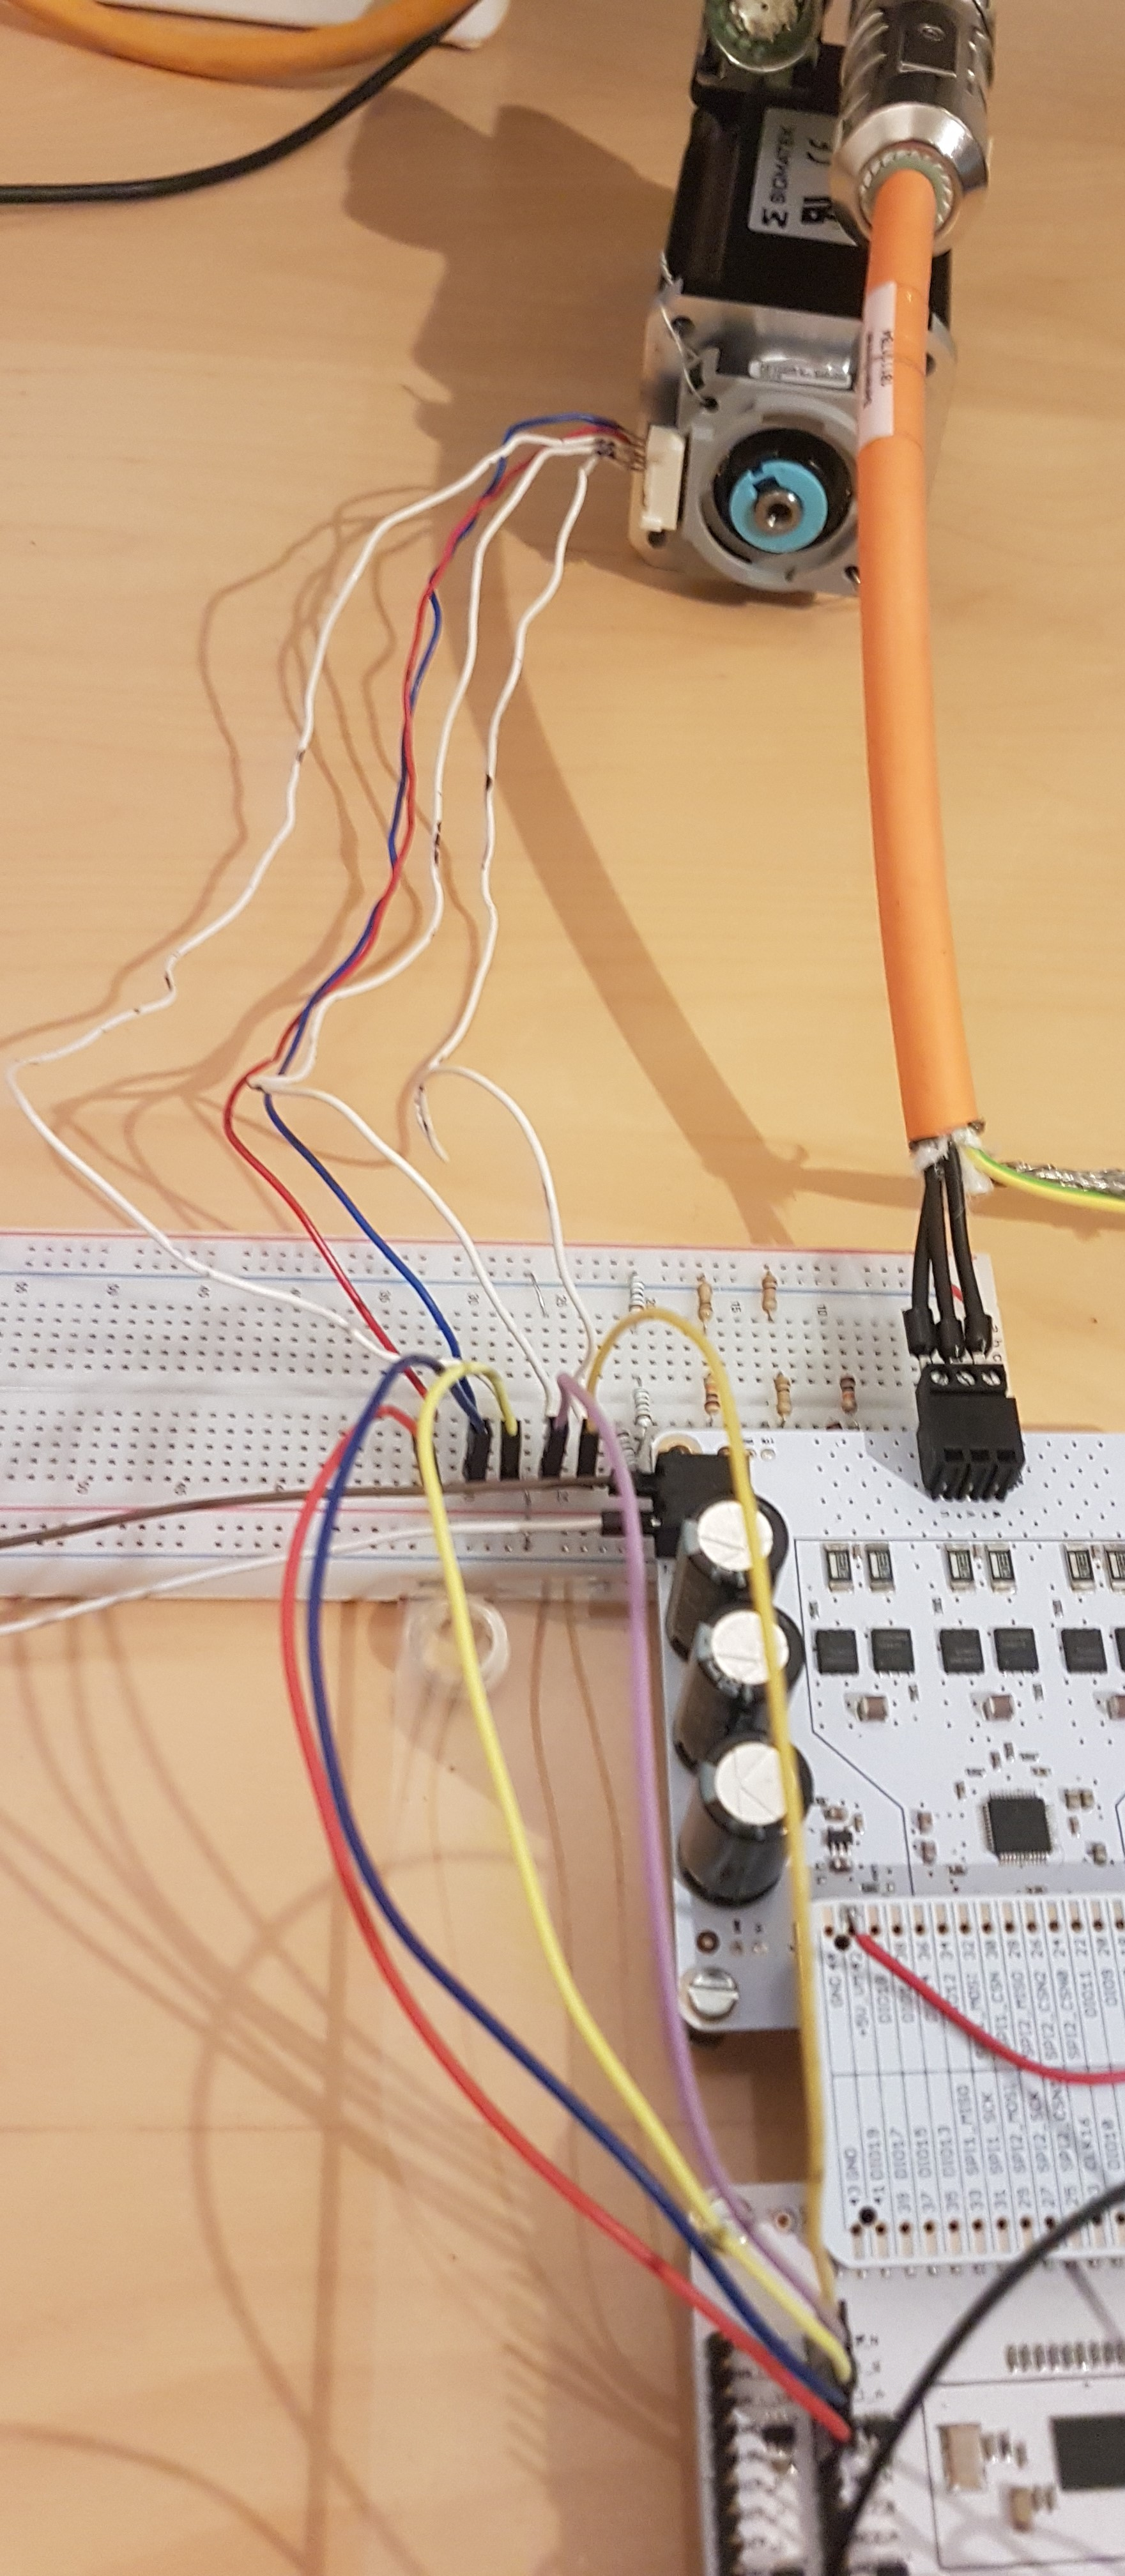
\includegraphics[angle = 270, width=\textwidth]{graphics/4_Antriebskette}
	\caption{Encoder-Interface Pinout-Table.}
	\label{fig:4_Antriebskette}
\end{figure}

\begin{figure}[H]
	\centering
	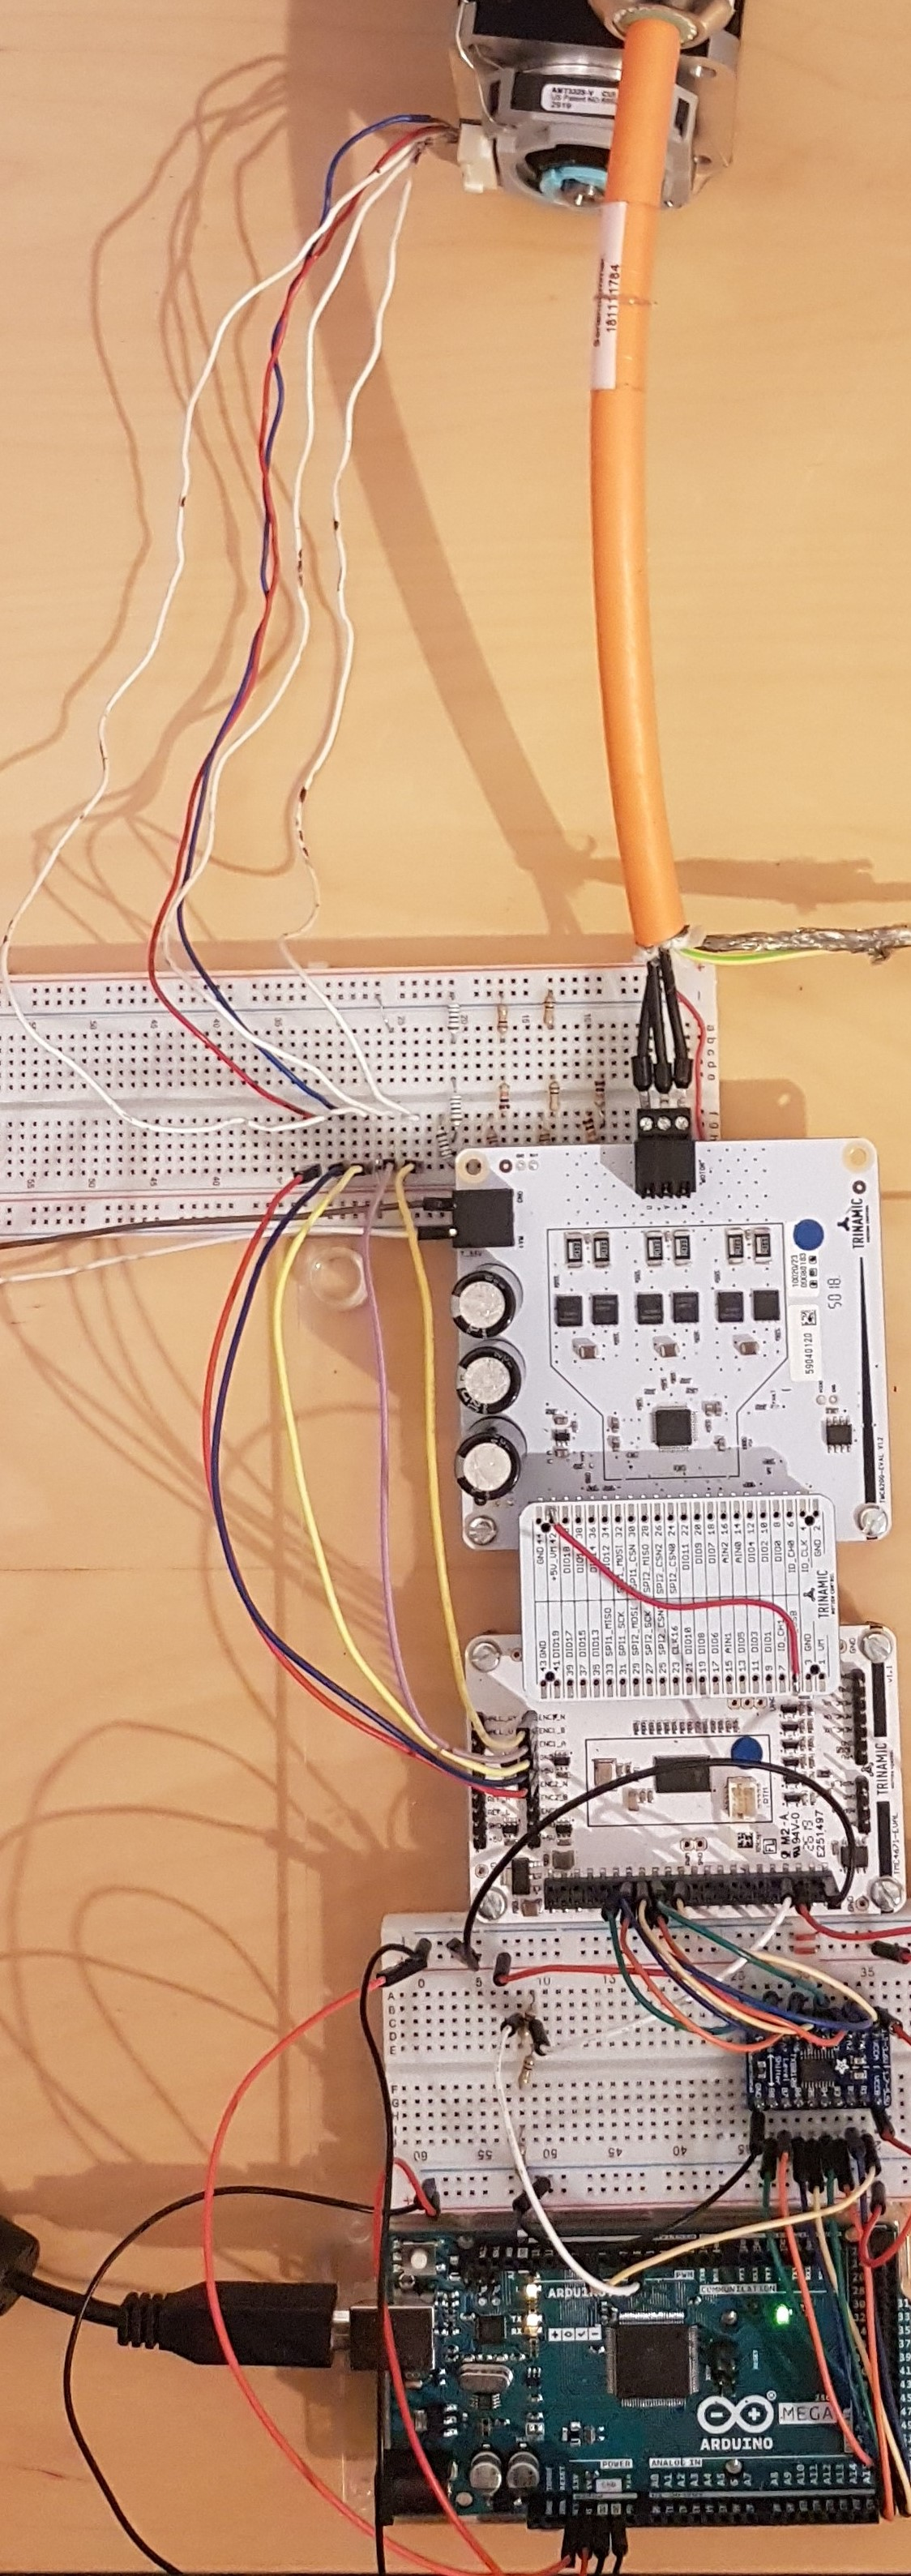
\includegraphics[angle = 270, width=\textwidth]{graphics/4_komplett}
	\caption{Encoder-Interface Pinout-Table.}
	\label{fig:4_komplett}
\end{figure}

\begin{figure}[H]
	\centering
	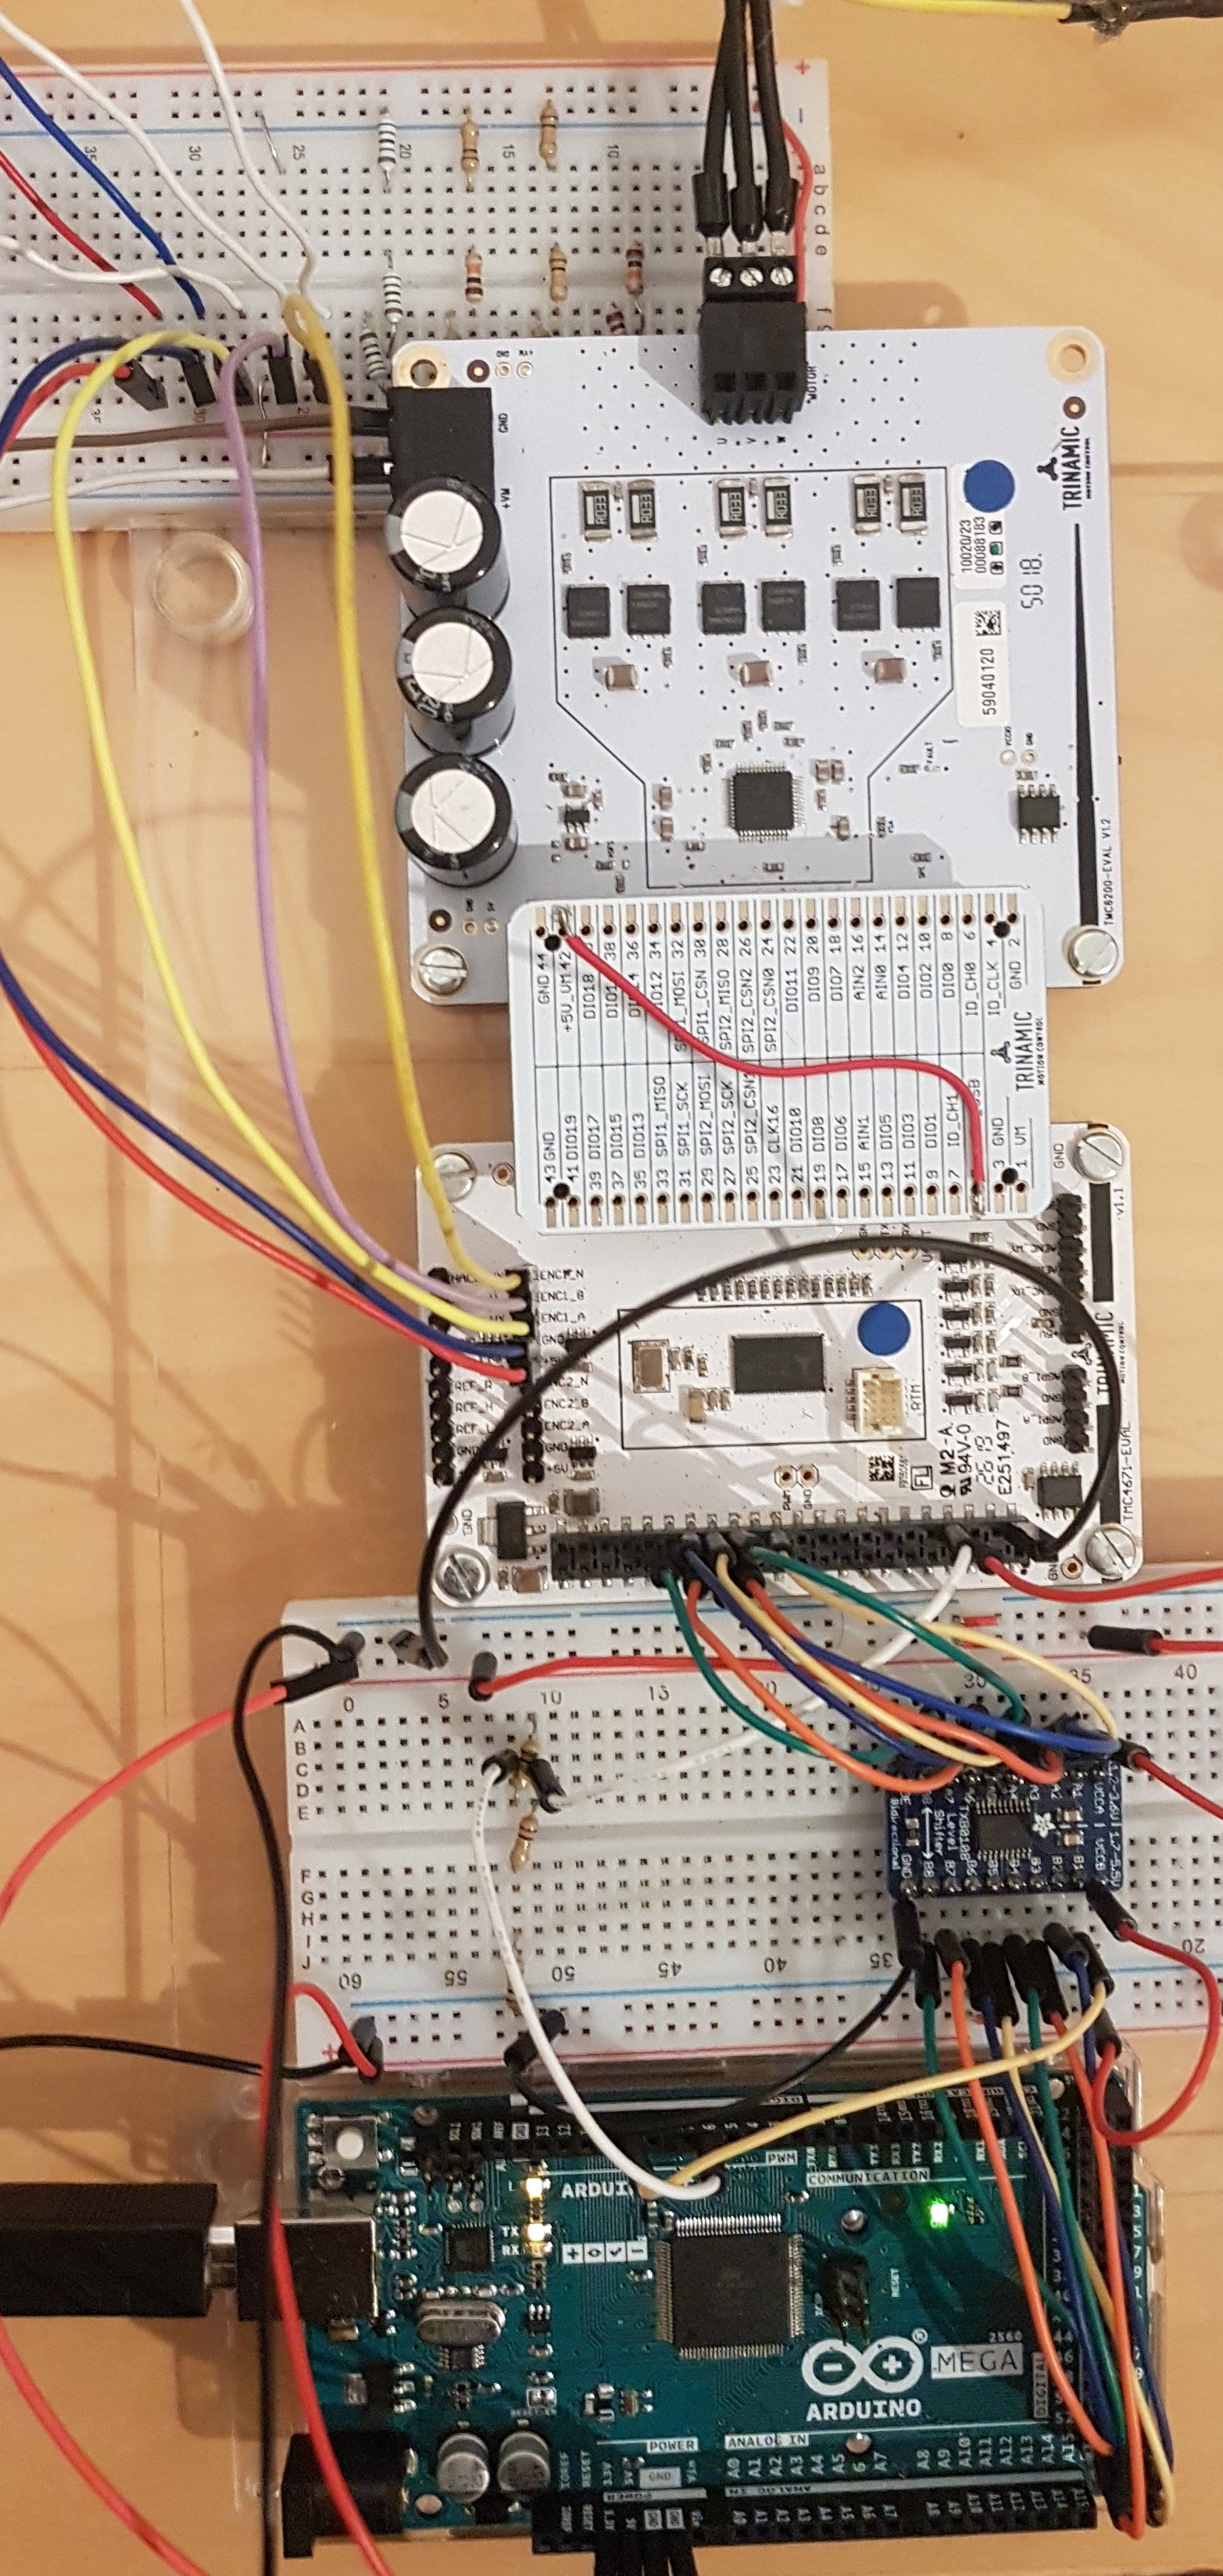
\includegraphics[angle = 270, width=\textwidth]{graphics/4_Elektronik}
	\caption{Encoder-Interface Pinout-Table.}
	\label{fig:4_Elektronik}
\end{figure}


\subsubsection{Encoder-Signale}\label{Appendix:ABN_Signale}

\begin{figure}[H]
	\centering
	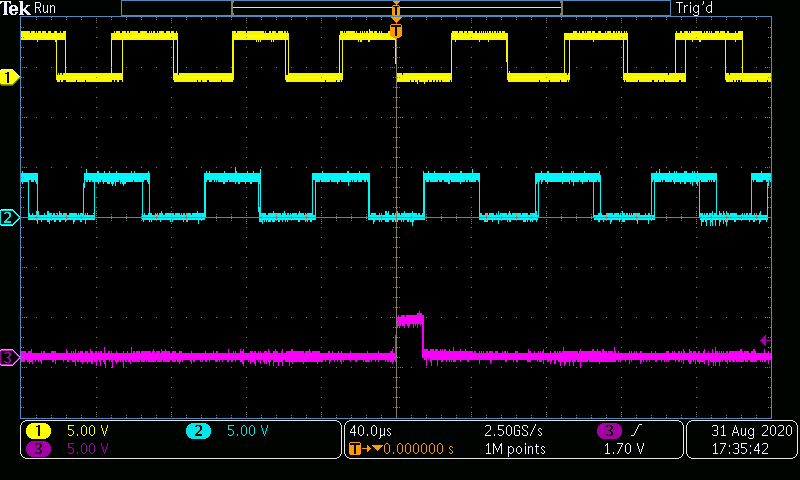
\includegraphics[width=\textwidth]{graphics/AMT322S-V_Signal}
	\caption{Encoder-Interface Pinout-Table. Gelb = A, Blau = B, N = Magenta}
	\label{fig:AMT322S-V_Signal}
\end{figure}
